%!TEX root = practicum2.tex
\todo[inline]{Inleiding in experiment}


\subsection{Probability}
\label{ss:exp:probability}
	\todo[inline]{Discuss cluster size statistics, mean cluster size M and sd as a function p for finite clusters}
	\todo[inline]{Determine some vague fraction}

To investigate the effect of different $p$ on a lattice with a constant size we perform the following experiment. We opt for a lattice size, with $N = 20$, which results in $41 \times 41$ sized grid. We calculate the mean and standard deviation over $r_{max} = 200$, with the range of $p$ between $0.3$ and $0.7$.

\begin{figure*}
	\centering
	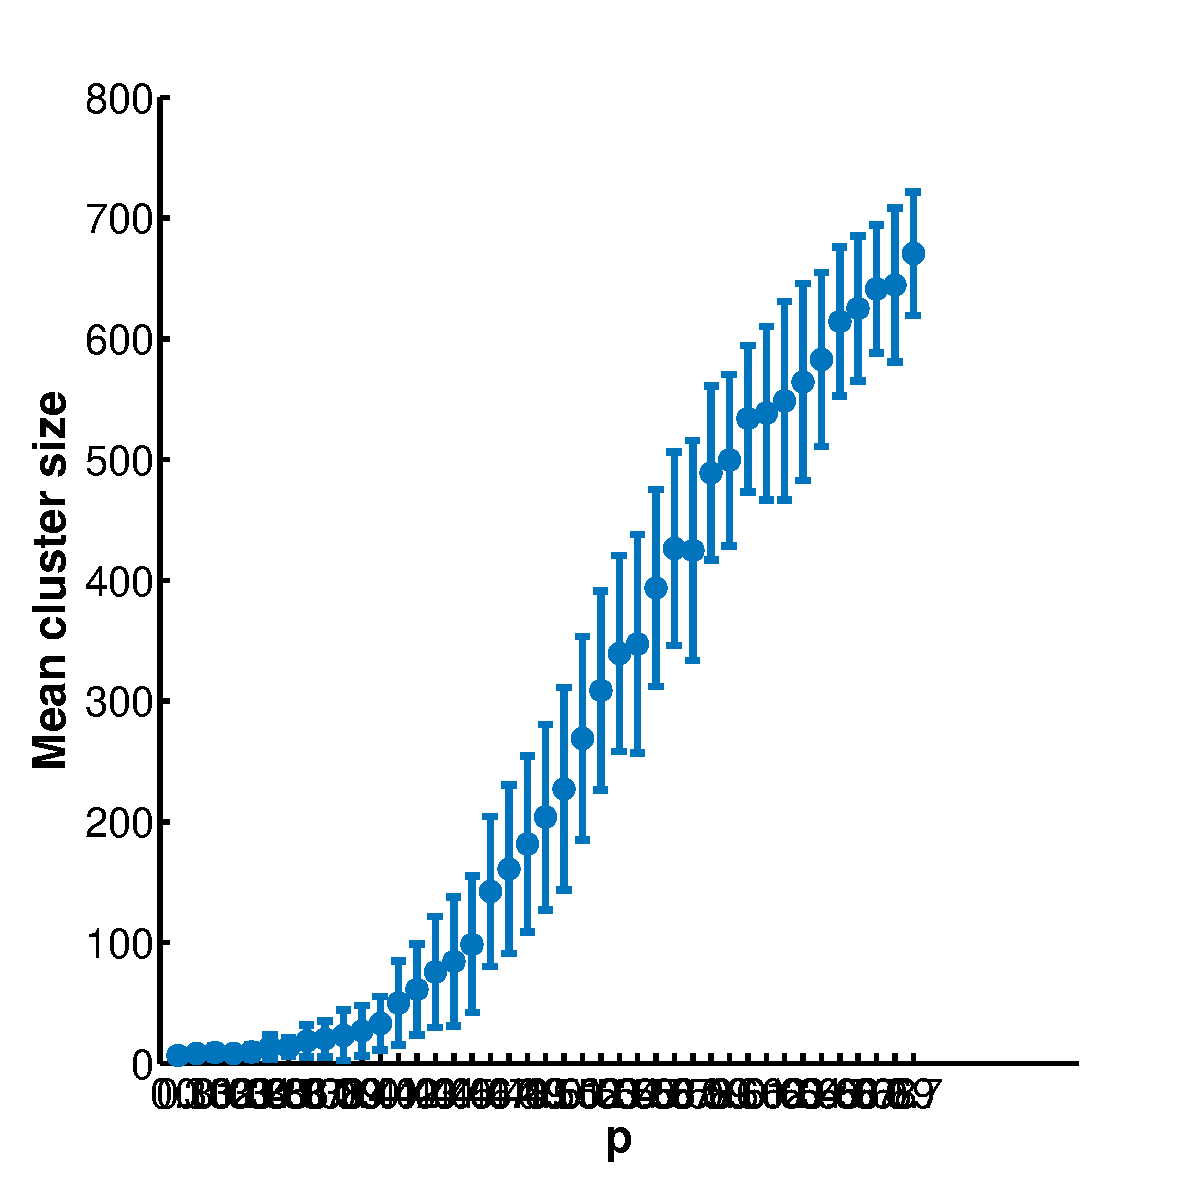
\includegraphics[width=\textwidth]{./img/assignment_a_mean_std_p.pdf}
	\caption{Mean cluster sizes $\mu$ (indicated by the points) and standard deviations $\sigma$ (vertical error bars) computed as a function of p, with a step size of $0.01$. Values $\mu$ and $\sigma$ were calculated over $200$ runs with a grid of size $41 \times 41$.}
	\label{fig:experiment:mean_std_clusters}
\end{figure*}

\begin{figure}
	\centering
	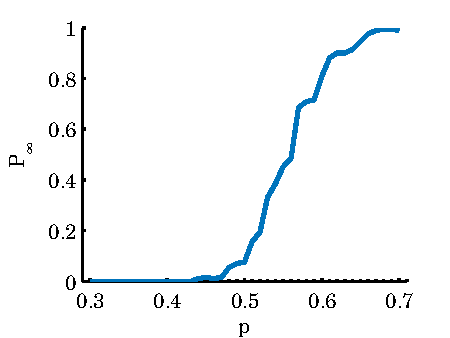
\includegraphics[width=\columnwidth]{./img/assignment_a_p_infinite_ratio_p.pdf}
	\caption{Caption here}
	\label{fig:experiment:p_inf_ratio}
\end{figure}

\subsection{System Size}
\label{ss:exp:systemSize}
	\todo[inline]{How do the results change when the system size changes. Experiment with different latice sizes}
	\todo[inline]{Wat could the behavior be in the limit of infinite lattice sizes}

\subsection{Fractal Dimension}
\label{ss:exp:fractal}
	\todo[inline]{Bonus: Determine the fractal dimension of finite clusters as a function of $p$.}

\subsection{Connectivity}
\label{ss:exp:connectivity}
	\todo[inline]{Present mask used previously, and 8-connected mask}
	\todo[inline]{How does the connectivity influence the final cluster}
